\documentclass[12pt,a4paper]{article}

\usepackage[margin=2.5cm]{geometry}
\usepackage[utf8]{inputenc}
\usepackage[T1]{fontenc}
\usepackage{helvet}
\renewcommand{\familydefault}{\sfdefault}
\usepackage[spanish,es-nodecimaldot]{babel}
\usepackage{graphicx}
\graphicspath{{imagenes/}}
\usepackage{float}
\usepackage{caption}
\usepackage{setspace}
\usepackage{titlesec}
\usepackage{fancyhdr}
\usepackage{ragged2e}
\usepackage{indentfirst}
\usepackage{enumitem}
\usepackage[hidelinks]{hyperref}
\usepackage{xurl}
\urlstyle{same}

\setlength{\parindent}{1.27cm}
\setlength{\parskip}{0pt}
\setlength{\headheight}{15pt}
\setcounter{tocdepth}{2}
\setcounter{secnumdepth}{2}

\titleformat{\section}
  {\bfseries\fontsize{14}{17}\selectfont\raggedright}
  {\thesection}{0.8em}{}
\titleformat{name=\section,numberless}
  {\bfseries\fontsize{14}{17}\selectfont\raggedright}
  {}{0pt}{}
\titleformat{\subsection}
  {\bfseries\fontsize{12}{15}\selectfont\raggedright}
  {\thesubsection}{0.8em}{}
\titlespacing*{\section}{0pt}{18pt}{10pt}
\titlespacing*{\subsection}{0pt}{14pt}{7pt}

\captionsetup{
  font={small,stretch=1.0},
  labelfont=bf,
  labelsep=period,
  justification=centering,
  singlelinecheck=false
}
\renewcommand{\figurename}{Figura}
\renewcommand{\contentsname}{Índice}
\addto\captionsspanish{\renewcommand{\listfigurename}{Índice de imágenes}}

\fancypagestyle{contenido}{
  \fancyhf{}
  \fancyhead[R]{\thepage}
  \renewcommand{\headrulewidth}{0pt}
  \renewcommand{\footrulewidth}{0pt}
}

\newcommand{\entradafrancesa}[1]{%
  \par\noindent
  \hangindent=1.27cm
  \hangafter=1
  #1\par
}

\begin{document}

\pagenumbering{Alph}

\begin{titlepage}
  \centering
  \vspace*{1.2cm}
  
\includegraphics[width=0.20\textwidth]{logo_upp.png}

  \vspace{1.0cm}
  {\bfseries\fontsize{14}{17}\selectfont Universidad Politécnica de Pachuca\par}
  \vspace{0.8cm}
  {\bfseries\fontsize{14}{17}\selectfont Desarrollo de Aplicaciones Móviles\par}
  \vspace{0.8cm}
  {\bfseries\fontsize{14}{17}\selectfont Diálogos con Jetpack Compose\par}
  \vspace{0.3cm}
  {\bfseries\fontsize{12}{15}\selectfont Práctica\par}

  \vspace{1.2cm}
  {\bfseries Autor:\par}
  \vspace{0.25cm}
  Cabrera Bardales Edgar Alejandro\par
  \vspace{0.2cm}
  2531126226\par

  \vspace{0.8cm}
  {\bfseries Profesor:\par}
  \vspace{0.25cm}
  Ing. Montoya Cerro Miguel Ángel\par

  \vspace{0.8cm}
  {\bfseries Grupo:\par}
  \vspace{0.25cm}
  TIID 04-01\par

  \vfill
  Zempoala, Hidalgo, México a 09 de noviembre de 2026\par
\end{titlepage}

\pagenumbering{roman}
\pagestyle{empty}
\begingroup
\setstretch{1.15}
\tableofcontents
\clearpage
\listoffigures
\endgroup
\clearpage

\pagenumbering{arabic}
\pagestyle{contenido}
\RaggedRight
\doublespacing

\section{Introducción}

En el desarrollo de aplicaciones móviles para Android, los diálogos permiten mostrar información importante o solicitar una decisión sin abandonar la pantalla actual. Jetpack Compose incorpora componentes de Material 3 que facilitan esta tarea mediante una estructura declarativa. De esta manera, el título, el mensaje y las acciones se organizan dentro de una función composable y se actualizan según el estado de la interfaz.

La presente práctica tiene como objeto de estudio la creación de un cuadro de confirmación mediante AlertDialog. El procedimiento comienza con un proyecto Empty Activity generado en Android Studio. Posteriormente, se elimina el contenido de ejemplo, se construye una pantalla con un botón centrado y se agrega un diálogo personalizado con el título ODEG jugando Granny y dos respuestas posibles.

Finalmente, se utiliza una variable booleana para controlar la visibilidad del cuadro. El botón principal cambia el estado para mostrarlo, mientras que las acciones Sí y No ejecutan funciones diferentes. Las diez evidencias obtenidas en Android Studio permiten observar el avance desde el proyecto inicial hasta el diálogo final funcionando en el emulador Pixel 5.

\section{Objetivos}

\subsection{Objetivo central}

Implementar un diálogo de confirmación en Android Studio mediante Kotlin, Jetpack Compose y Material 3, controlando su visibilidad y sus acciones a través de un estado observable.

\subsection{Objetivos específicos}

\begin{itemize}[leftmargin=1.2cm]
  \item Crear una pantalla básica que muestre un botón centrado dentro del espacio disponible.
  \item Construir un AlertDialog con título, mensaje y botones de confirmación y cancelación.
  \item Utilizar remember y mutableStateOf para mostrar u ocultar el diálogo durante la ejecución.
  \item Conectar las funciones de cierre y confirmación con las acciones disponibles en el cuadro.
  \item Comprobar el resultado de cada etapa mediante el emulador integrado en Android Studio.
\end{itemize}

\section{Justificación}

Esta práctica resulta relevante porque los diálogos aparecen con frecuencia en aplicaciones que necesitan confirmar una acción, presentar una advertencia o solicitar una selección. Su uso permite mantener al usuario dentro del contexto actual y concentrar la atención en una decisión específica. Comprender su estructura facilita incorporar mensajes de confirmación sin crear una actividad adicional.

Asimismo, el ejercicio permite reforzar el manejo de estados en Jetpack Compose. El diálogo no debe permanecer visible de manera permanente, sino reaccionar al botón que lo abre y a las acciones que lo cierran. Esta relación entre estado y eventos constituye una parte fundamental del modelo declarativo utilizado para construir interfaces en Android.

\section{Estructura del documento}

El presente documento se organiza en cinco partes principales. La primera contiene la introducción, los objetivos y la justificación de la práctica. La segunda presenta el marco teórico relacionado con AlertDialog, los botones de Material 3, el estado y el flujo de eventos. La tercera sección describe el desarrollo paso a paso mediante las diez evidencias obtenidas en Android Studio. Finalmente, se presentan las conclusiones, las recomendaciones, el anexo con el video consultado y las referencias oficiales utilizadas.

\section{Marco teórico}

\subsection{Diálogos en Jetpack Compose}

Un diálogo se muestra sobre el contenido principal de la aplicación y dirige la atención del usuario hacia un mensaje o una decisión. La documentación oficial indica que puede utilizarse para confirmar acciones, solicitar información o presentar opciones. Dentro de Jetpack Compose, AlertDialog ofrece una estructura preparada para integrar un título, un texto y acciones de confirmación o cancelación (Android Developers, 2026a).

El parámetro onDismissRequest se ejecuta cuando el usuario solicita cerrar el cuadro, por ejemplo, al tocar fuera de él o utilizar la acción Atrás. Los espacios confirmButton y dismissButton reciben componentes composables, por lo que en esta práctica se utilizan botones de texto para representar las opciones Sí y No.

\subsection{Botones y acciones}

Los botones permiten que el usuario ejecute una acción definida por la aplicación. El componente Button se utiliza para la acción principal que abre el diálogo. Su parámetro onClick recibe una función que se ejecuta al pulsarlo. Por otra parte, TextButton presenta una acción de menor énfasis visual y resulta apropiado dentro de un cuadro de confirmación (Android Developers, 2026b).

En la aplicación se utiliza un botón relleno con el texto Diálogo en el centro de la pantalla. Dentro de AlertDialog se agregan dos TextButton. La opción Sí llama a la función de confirmación, mientras que No utiliza la función encargada de cerrar el cuadro.

\subsection{Estado y recomposición}

El estado representa un valor que puede cambiar durante la ejecución y que determina parte de la interfaz mostrada. Compose permite almacenar valores simples mediante remember y mutableStateOf. Cuando cambia un valor observado, las funciones que lo utilizan pueden recomponerse para reflejar el nuevo resultado (Android Developers, 2026c).

En esta práctica, showDialog inicia con el valor false. El diálogo no aparece mientras se mantenga ese valor. Al pulsar el botón central, el estado cambia a true y la condición de MyDialog permite mostrar AlertDialog. Cuando el usuario cierra o confirma la acción, el estado vuelve a false y el cuadro desaparece.

\subsection{Flujo de estado y eventos}

La arquitectura de interfaz de Compose propone que el estado fluya hacia los componentes y que los eventos regresen hacia el lugar encargado de modificarlo. Este comportamiento permite separar la función que presenta el diálogo de la pantalla que conserva su estado (Android Developers, 2026d).

MyDialog recibe el valor show y las funciones onDismiss y onConfirm. De esta manera, el componente no decide por sí mismo dónde se almacena el estado. DialogScreen conserva la variable, la modifica cuando ocurre una pulsación y envía el resultado actualizado al diálogo.

\section{Desarrollo}

\subsection{Revisión del proyecto inicial}

Para comenzar, creamos un proyecto llamado dialogos mediante la plantilla Empty Activity de Android Studio. La actividad contiene el tema de la aplicación, un Scaffold y la función Greeting generada automáticamente. Antes de realizar cambios se revisa esta estructura para reconocer el punto de entrada de la interfaz.

Como podemos observar en la figura 1, el proyecto se encuentra abierto en MainActivity.kt y todavía conserva el mensaje Hello Android. Esta evidencia establece el estado inicial antes de sustituir el contenido de ejemplo por la pantalla de la práctica.

\begin{figure}[H]
  \centering
  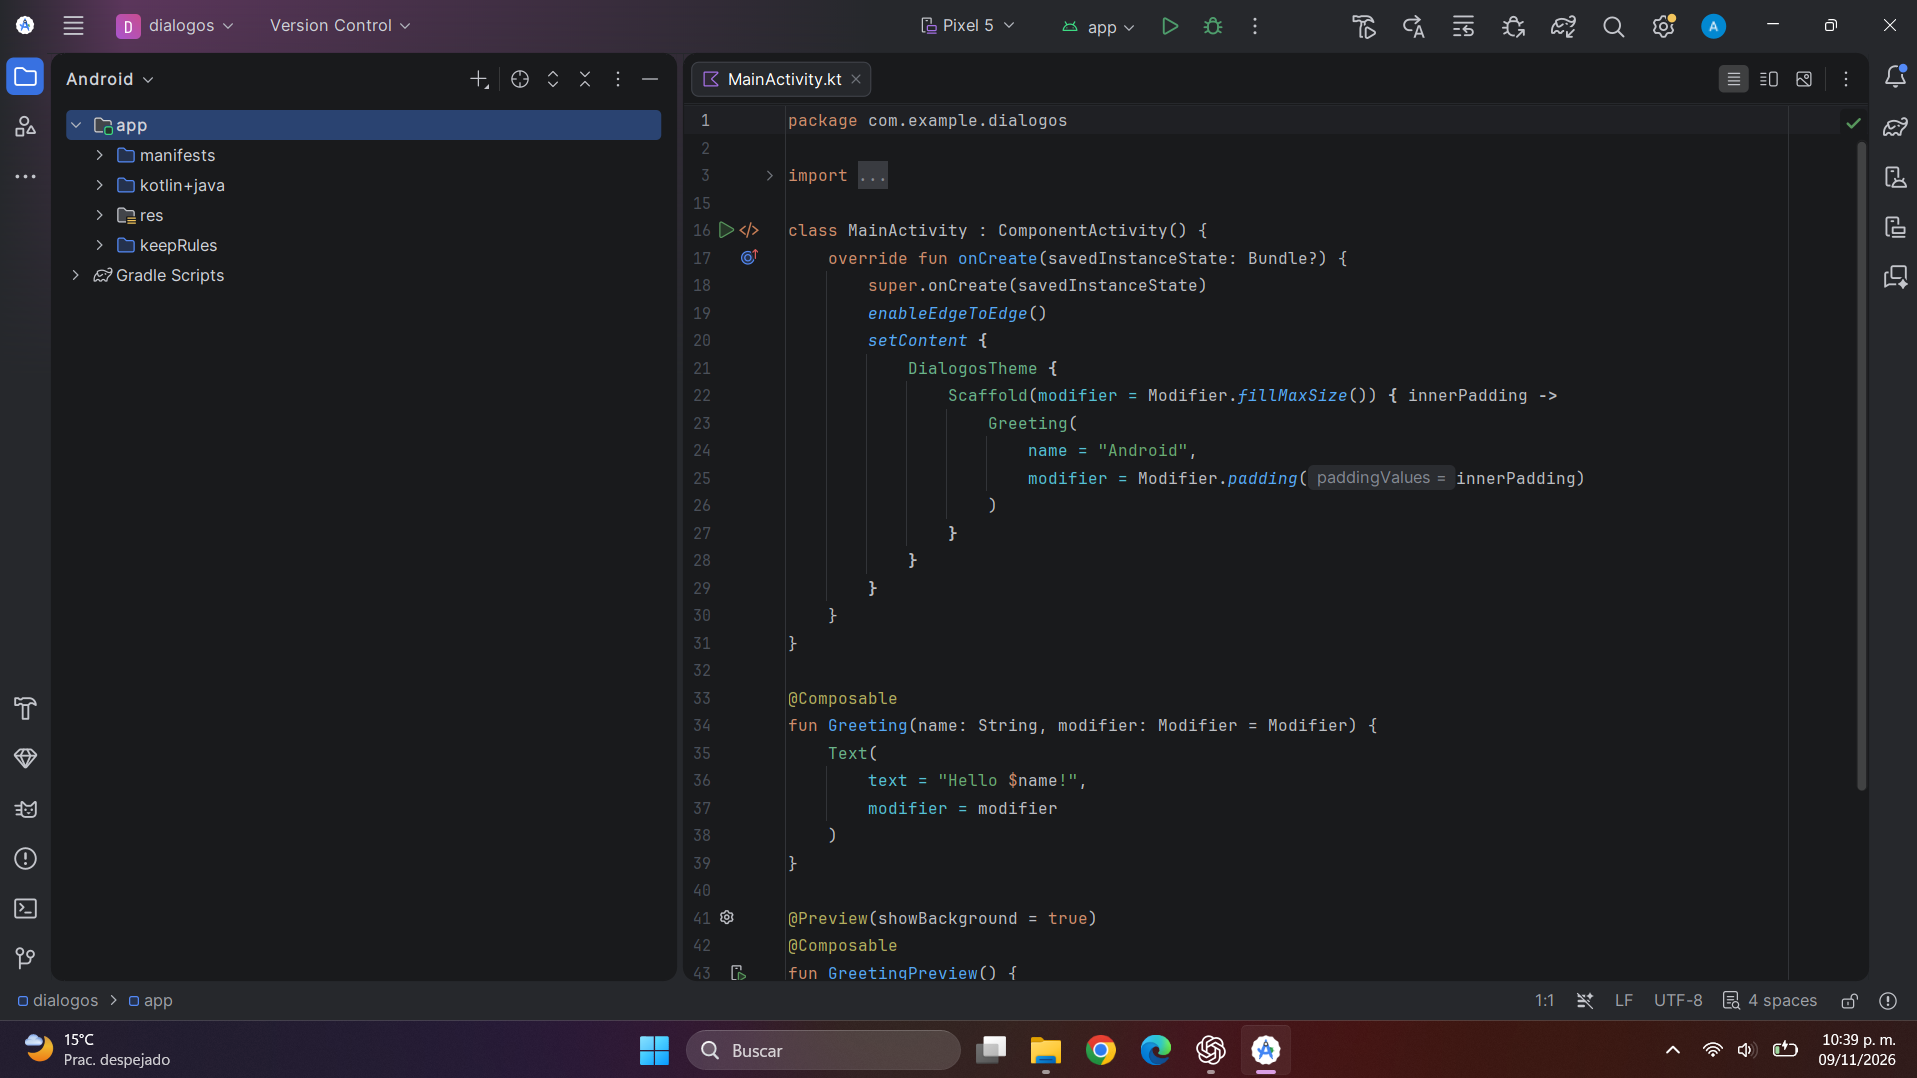
\includegraphics[width=\textwidth]{figura_01.png}
  \caption{Proyecto inicial}
\end{figure}

\subsection{Creación del botón centrado}

Posteriormente, eliminamos Greeting y creamos DialogScreen. Dentro de esta función agregamos un Box que ocupa el espacio disponible y establece la alineación central. En su contenido colocamos un Button con el texto Diálogo.

En la figura 2 podemos observar que el botón aparece en el centro del emulador. En esta etapa su acción se encuentra vacía, pues primero necesitamos construir el componente que será mostrado al pulsarlo.

\begin{figure}[H]
  \centering
  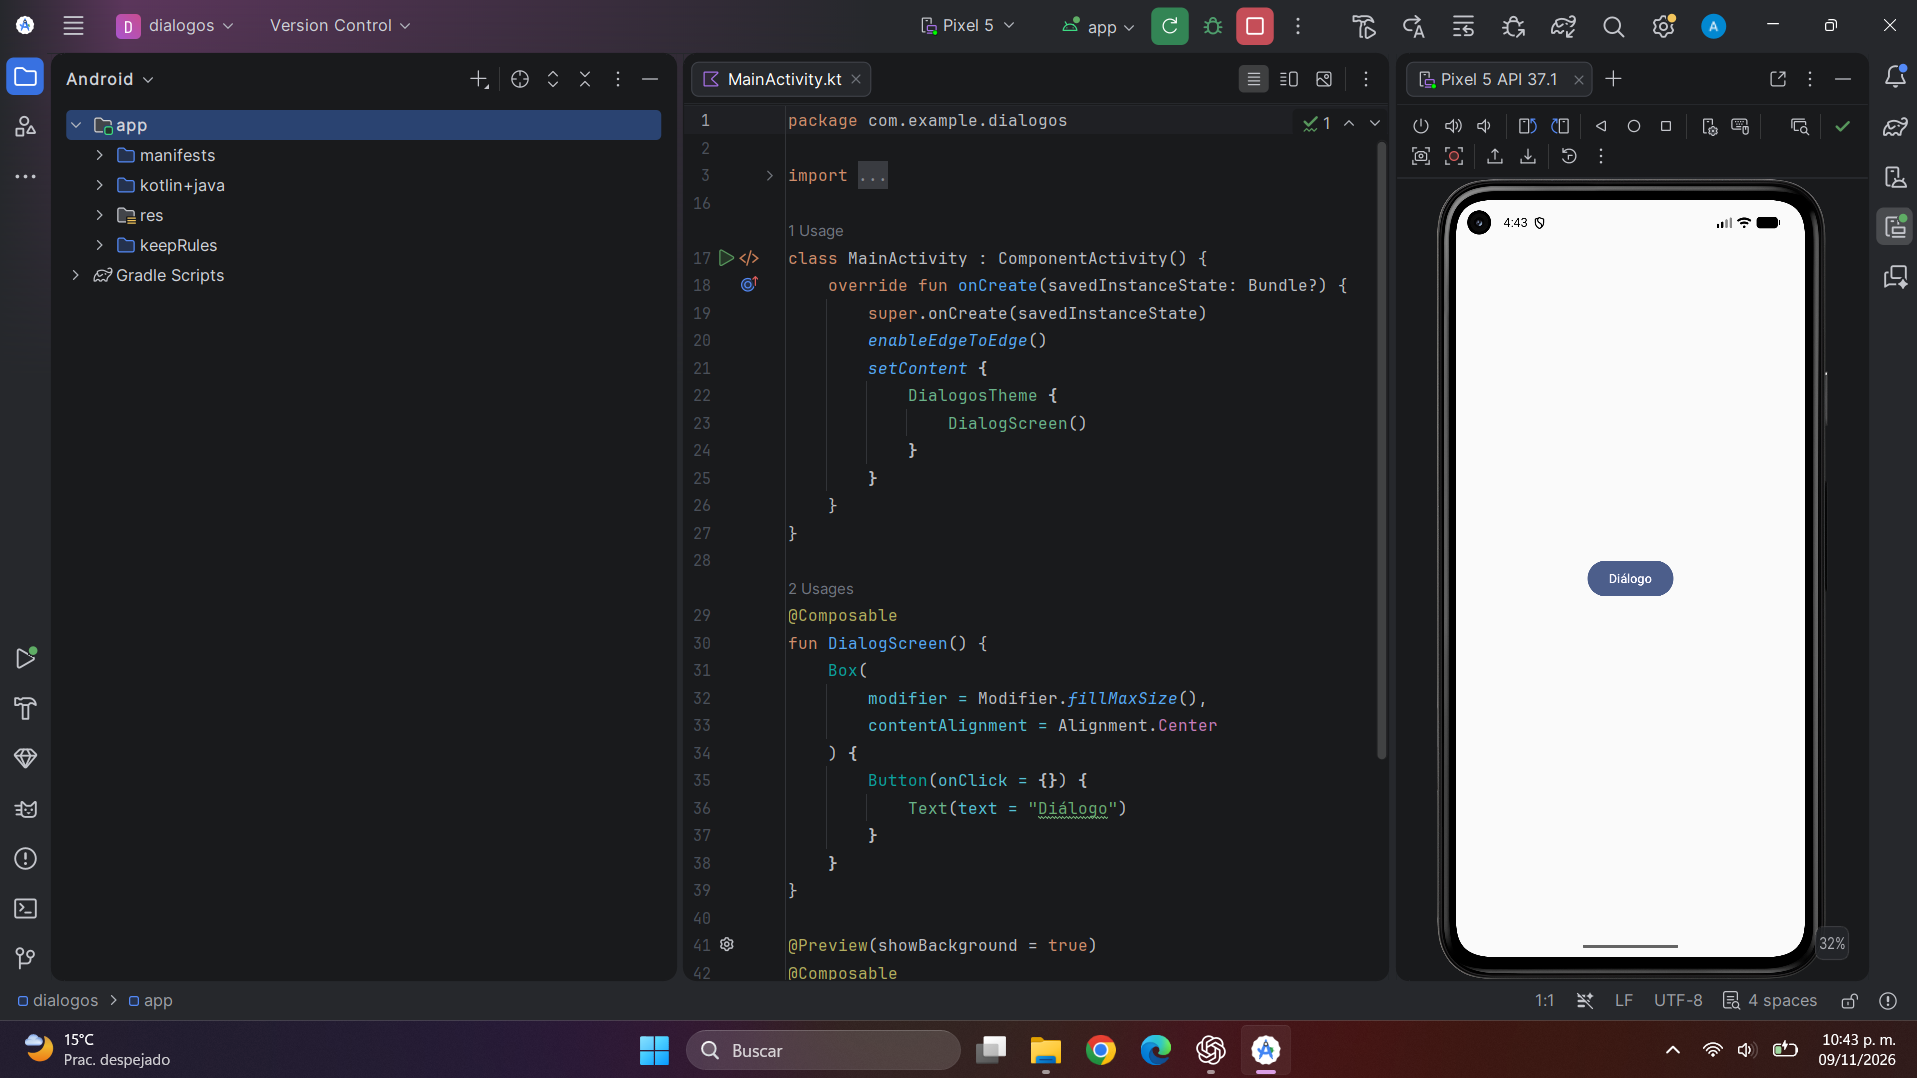
\includegraphics[width=\textwidth]{figura_02.png}
  \caption{Botón centrado}
\end{figure}

\subsection{Construcción del primer diálogo}

El siguiente paso consiste en declarar la función composable MyDialog. Dentro de ella agregamos AlertDialog y definimos el título ODEG jugando Granny junto con una pregunta relacionada. El espacio del botón de confirmación se mantiene vacío para comprobar primero la estructura básica.

Como se aprecia en la figura 3, el cuadro aparece sobre una capa oscura y concentra la atención en el mensaje. El botón principal continúa detrás del diálogo, aunque no puede utilizarse mientras el cuadro se encuentra activo.

\begin{figure}[H]
  \centering
  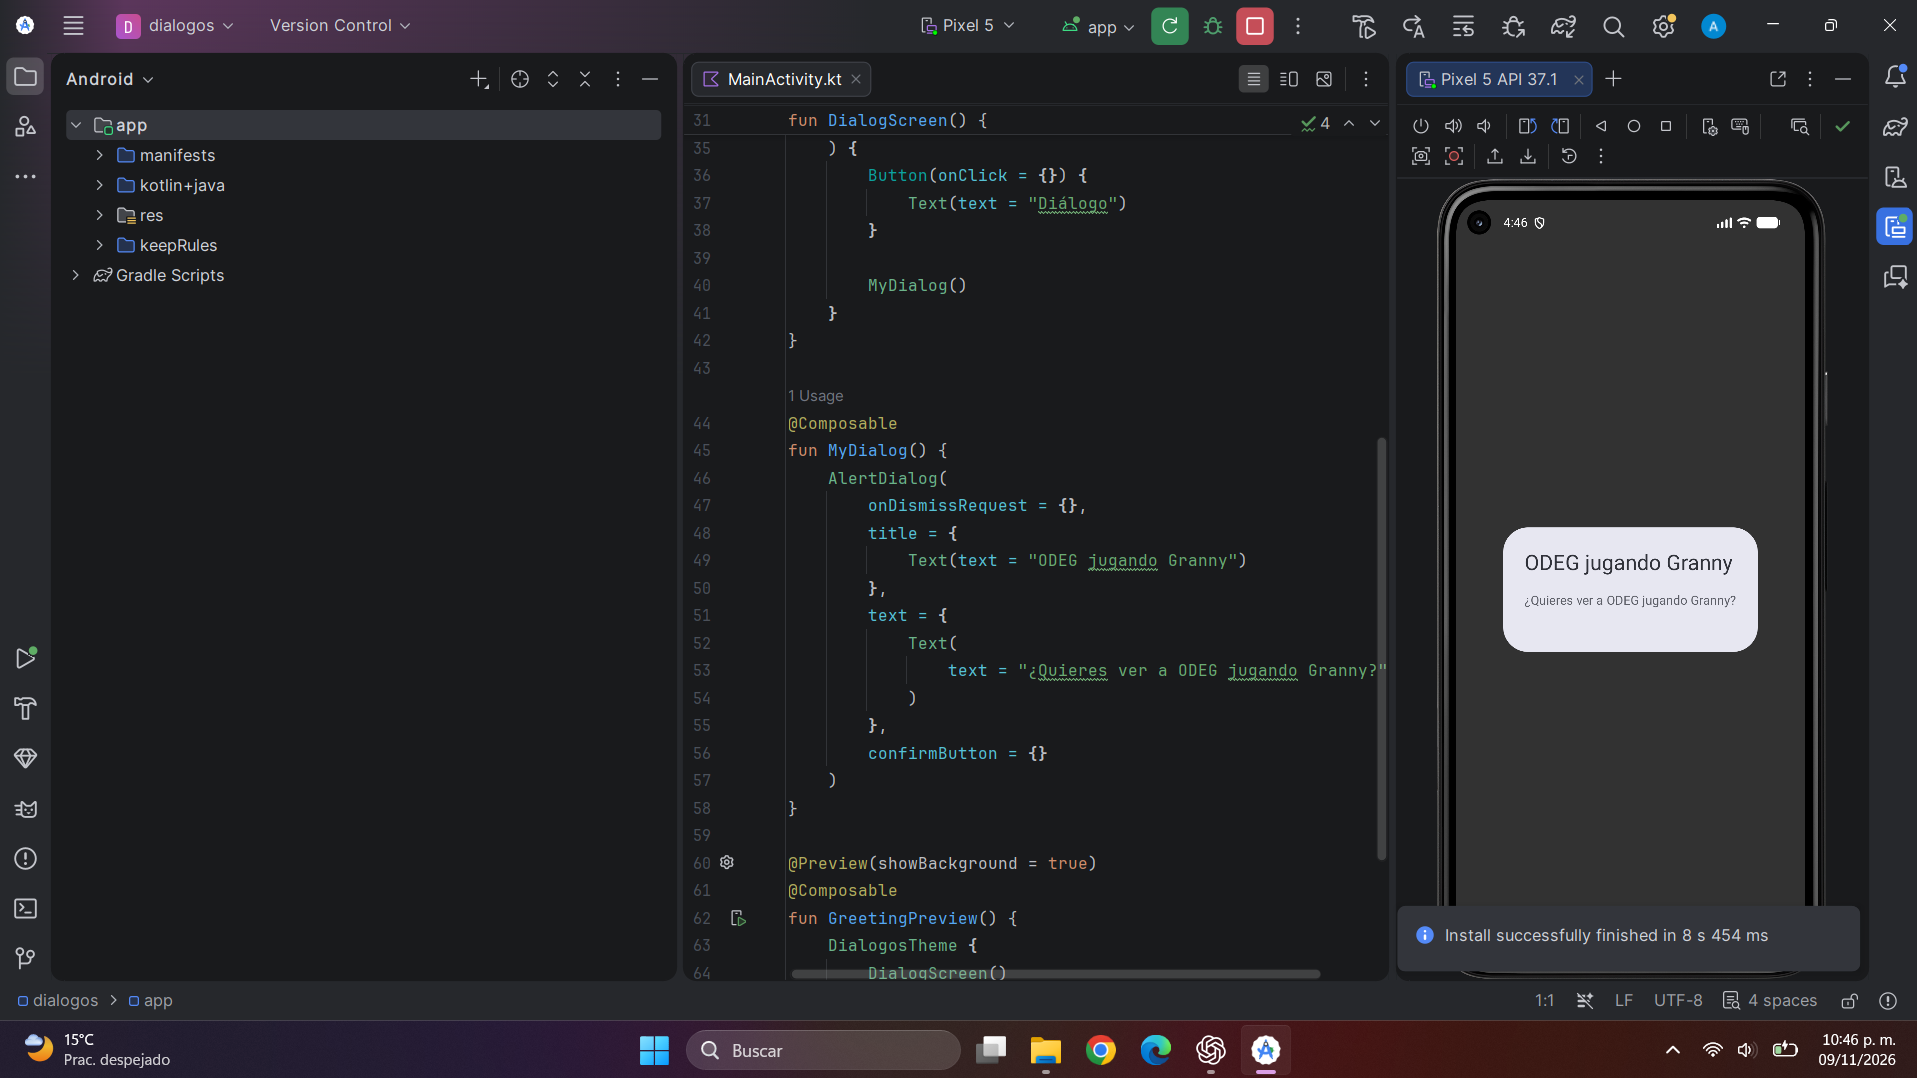
\includegraphics[width=\textwidth]{figura_03.png}
  \caption{Primer diálogo}
\end{figure}

\subsection{Incorporación de la confirmación}

Para agregar la primera respuesta, utilizamos el espacio confirmButton de AlertDialog. Dentro se coloca un TextButton con el texto Sí. Todavía no se conecta una acción, ya que en esta etapa únicamente se comprueba su presentación.

En la figura 4 podemos visualizar el botón en la parte inferior derecha del cuadro. La evidencia también muestra la sección de la función donde se declara el componente.

\begin{figure}[H]
  \centering
  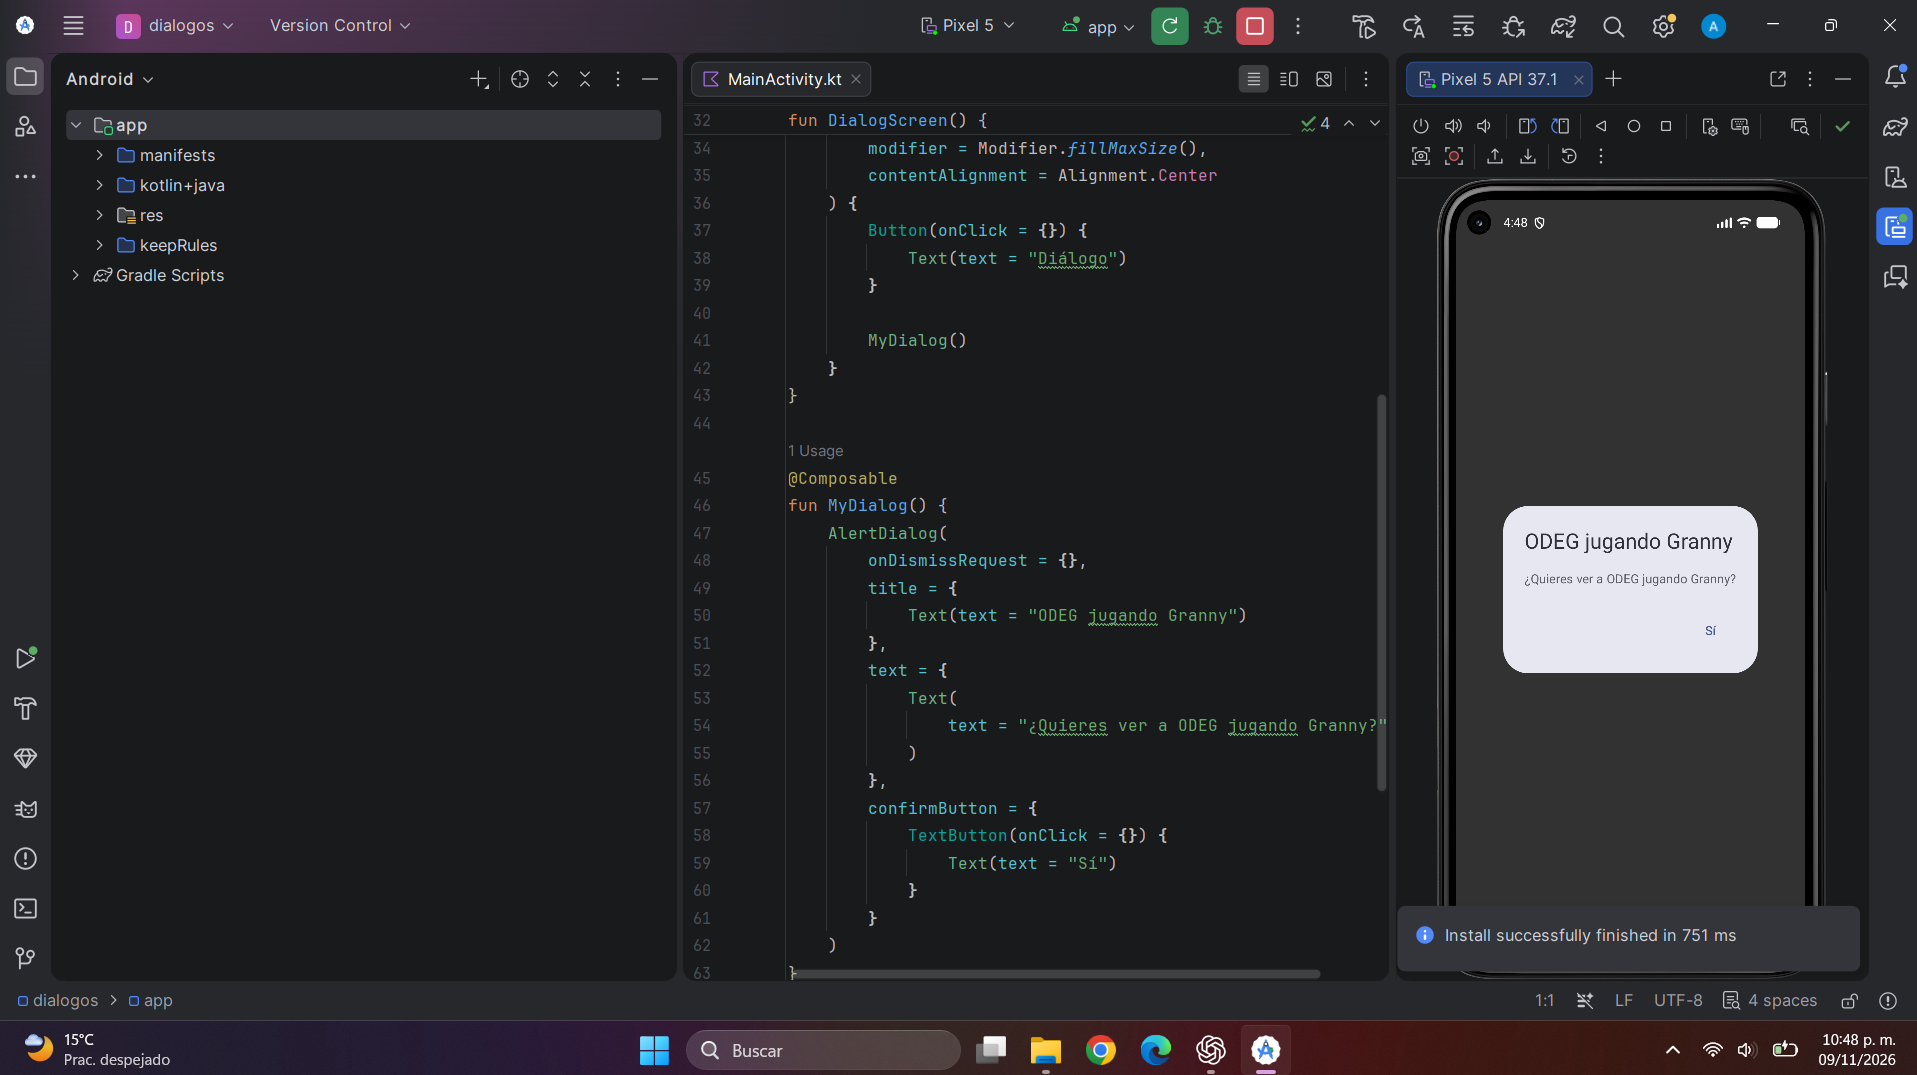
\includegraphics[width=\textwidth]{figura_04.png}
  \caption{Botón Sí}
\end{figure}

\subsection{Incorporación de la cancelación}

Después agregamos dismissButton y colocamos otro TextButton con el texto No. Con ello, el diálogo presenta las dos alternativas necesarias para una confirmación. En este momento ambas acciones permanecen vacías, por lo que el cuadro todavía se muestra de forma permanente.

Como podemos observar en la figura 5, las opciones No y Sí aparecen alineadas dentro del diálogo. Esta distribución permite distinguir la acción secundaria de la confirmación principal.

\begin{figure}[H]
  \centering
  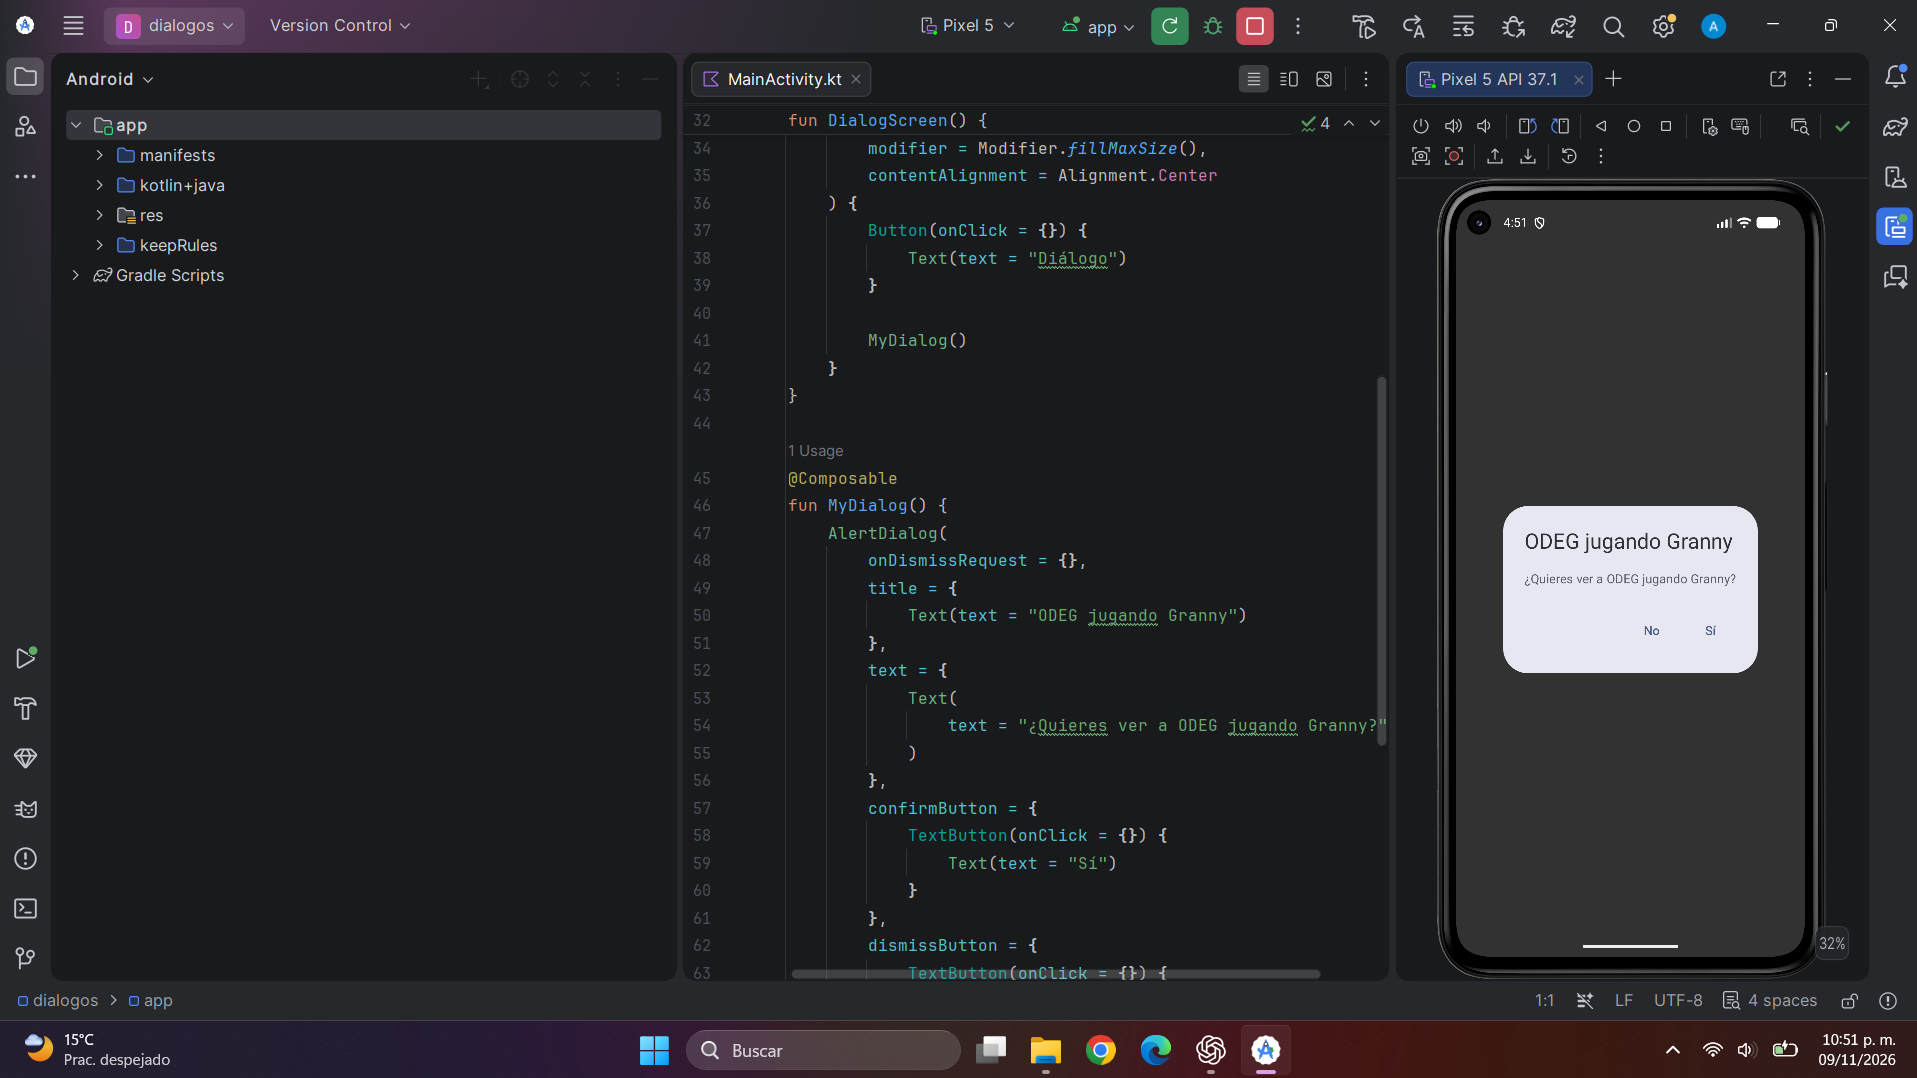
\includegraphics[width=\textwidth]{figura_05.png}
  \caption{Botones del diálogo}
\end{figure}

\subsection{Condición de visibilidad}

Para evitar que el cuadro se muestre siempre, MyDialog recibe un parámetro booleano llamado show. La estructura de AlertDialog se coloca dentro de una condición que solamente se ejecuta cuando el valor recibido es verdadero.

En la figura 6 podemos observar el parámetro y la condición. Durante esta comprobación se envía temporalmente el valor true, por lo que el diálogo permanece visible mientras verificamos que la nueva estructura compila correctamente.

\begin{figure}[H]
  \centering
  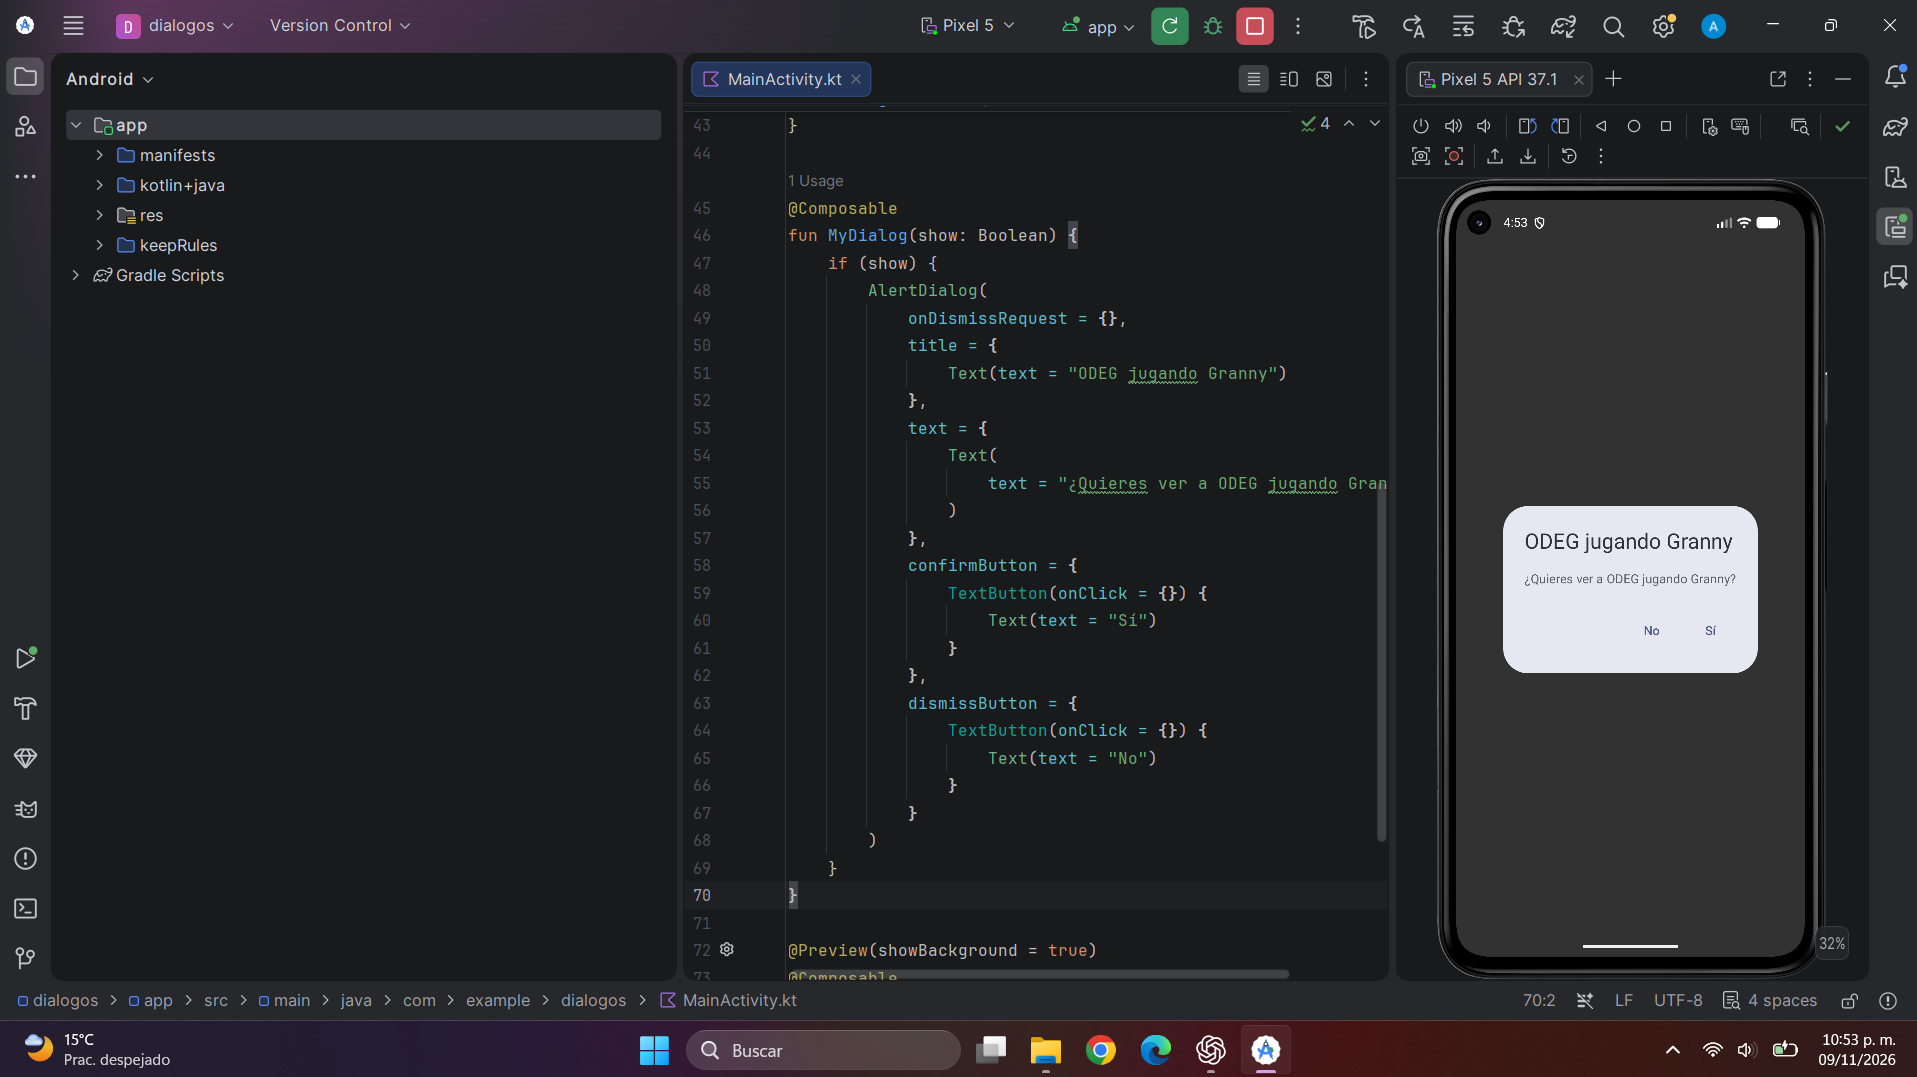
\includegraphics[width=\textwidth]{figura_06.png}
  \caption{Condición de visibilidad}
\end{figure}

\subsection{Creación del estado}

El valor fijo se sustituye por la variable showDialog, creada con remember y mutableStateOf. Su valor inicial es false para que la aplicación comience únicamente con el botón. La acción onClick cambia el estado a true y MyDialog recibe el valor actualizado.

Como se muestra en la figura 7, el cuadro ya no aparece durante la ejecución inicial. El código permite identificar la variable de estado, la acción del botón y la llamada al diálogo.

\begin{figure}[H]
  \centering
  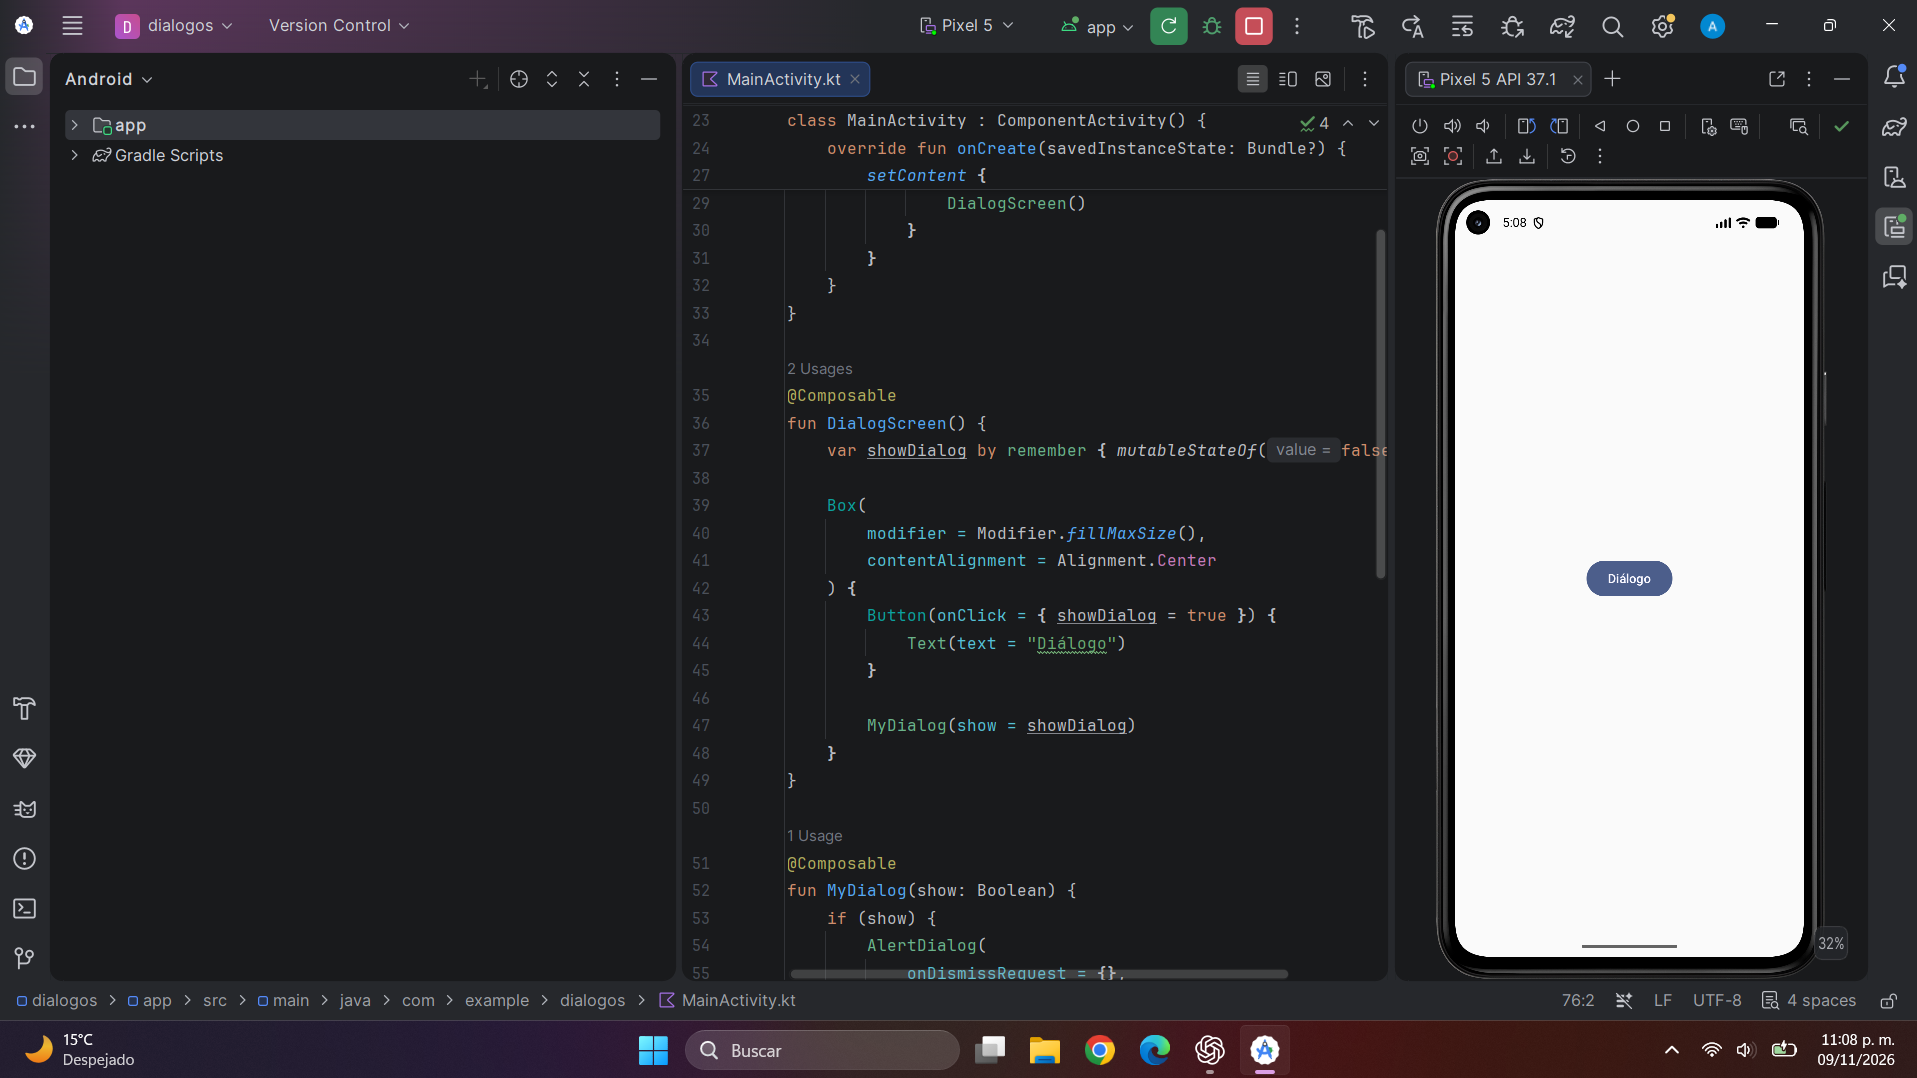
\includegraphics[width=\textwidth]{figura_07.png}
  \caption{Estado inicial}
\end{figure}

\subsection{Apertura del diálogo}

Posteriormente, pulsamos el botón Diálogo en el emulador. La acción cambia showDialog a true, Compose reconoce la modificación y vuelve a evaluar la parte de la interfaz que depende del valor. Como resultado, MyDialog cumple la condición y presenta AlertDialog.

En la figura 8 podemos observar el diálogo abierto y la relación entre el botón, el estado y la función que recibe el valor. Esta prueba confirma que la visibilidad ya no depende de un valor escrito directamente en la llamada.

\begin{figure}[H]
  \centering
  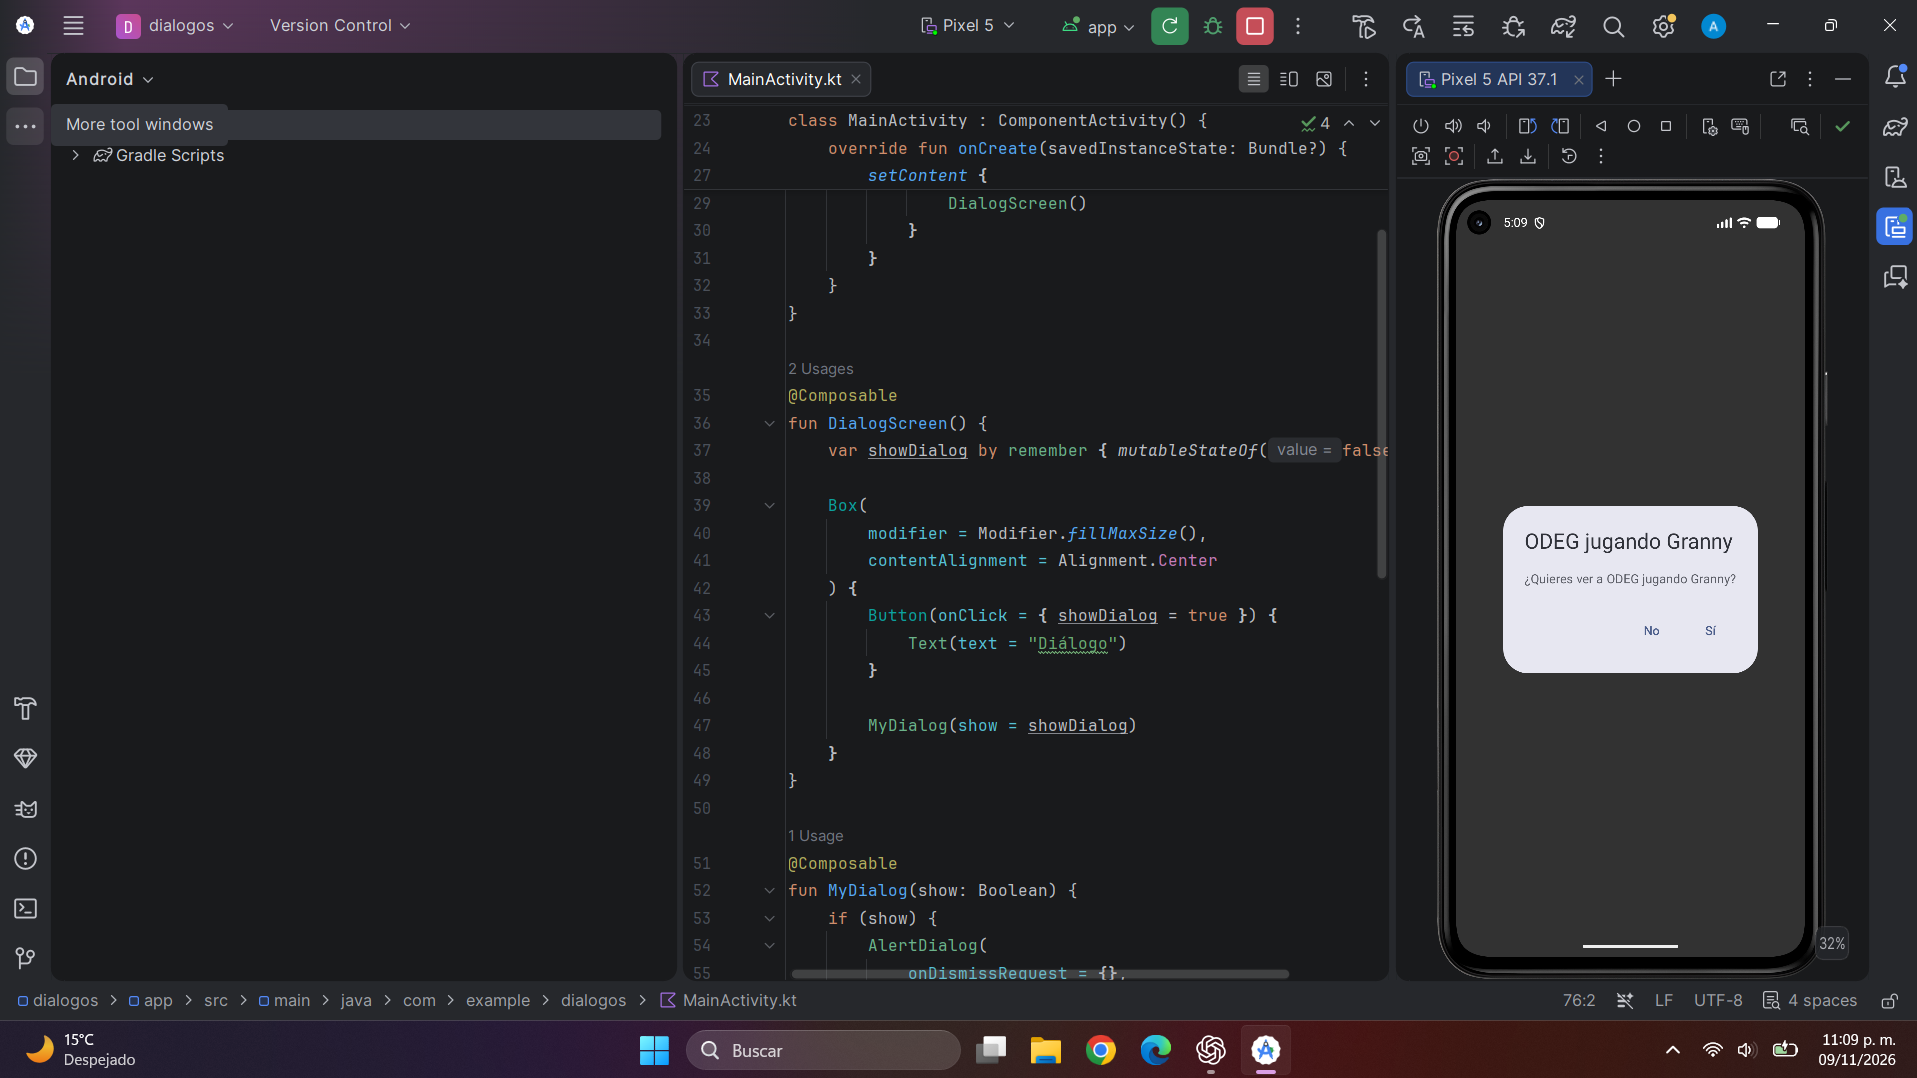
\includegraphics[width=\textwidth]{figura_08.png}
  \caption{Diálogo abierto}
\end{figure}

\subsection{Cierre mediante la opción No}

Para controlar el cierre, MyDialog recibe la función onDismiss. DialogScreen envía una acción que cambia showDialog a false. La misma función se conecta con onDismissRequest y con el botón No, permitiendo cerrar el cuadro de dos formas.

Como podemos observar en la figura 9, después de pulsar No la pantalla regresa al botón central. El código muestra que la acción de cancelación utiliza onDismiss para modificar el estado conservado por la pantalla.

\begin{figure}[H]
  \centering
  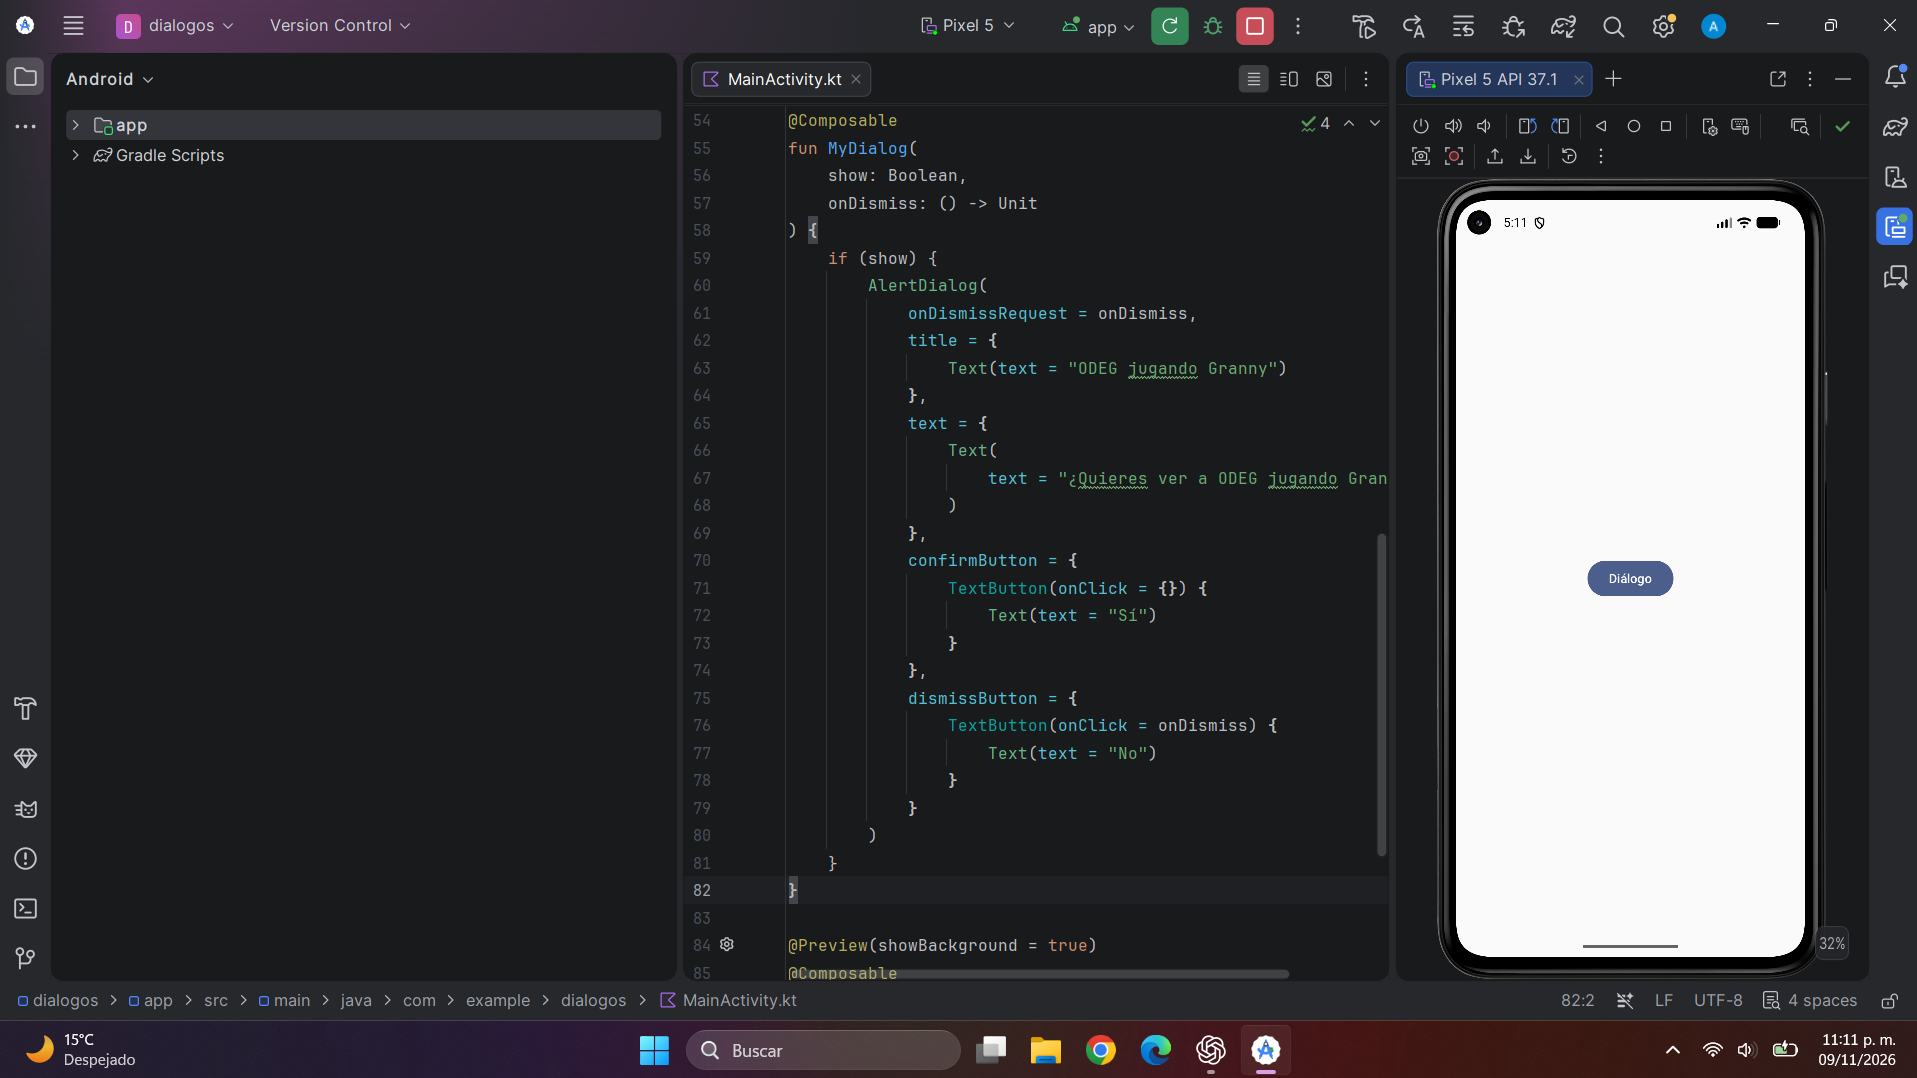
\includegraphics[width=\textwidth]{figura_09.png}
  \caption{Cierre con No}
\end{figure}

\subsection{Confirmación y resultado final}

Finalmente, agregamos la función onConfirm. Al pulsar Sí se registra el mensaje ODEG jugará Granny en Logcat y el estado vuelve a false. De esta manera, la confirmación ejecuta su propia acción y también cierra el cuadro.

En la figura 10 podemos visualizar el resultado final con ambas funciones conectadas. La opción Sí utiliza onConfirm y la opción No utiliza onDismiss. Después de probar las dos respuestas, el diálogo puede abrirse nuevamente desde el botón principal, con lo cual se completa el comportamiento solicitado.

\begin{figure}[H]
  \centering
  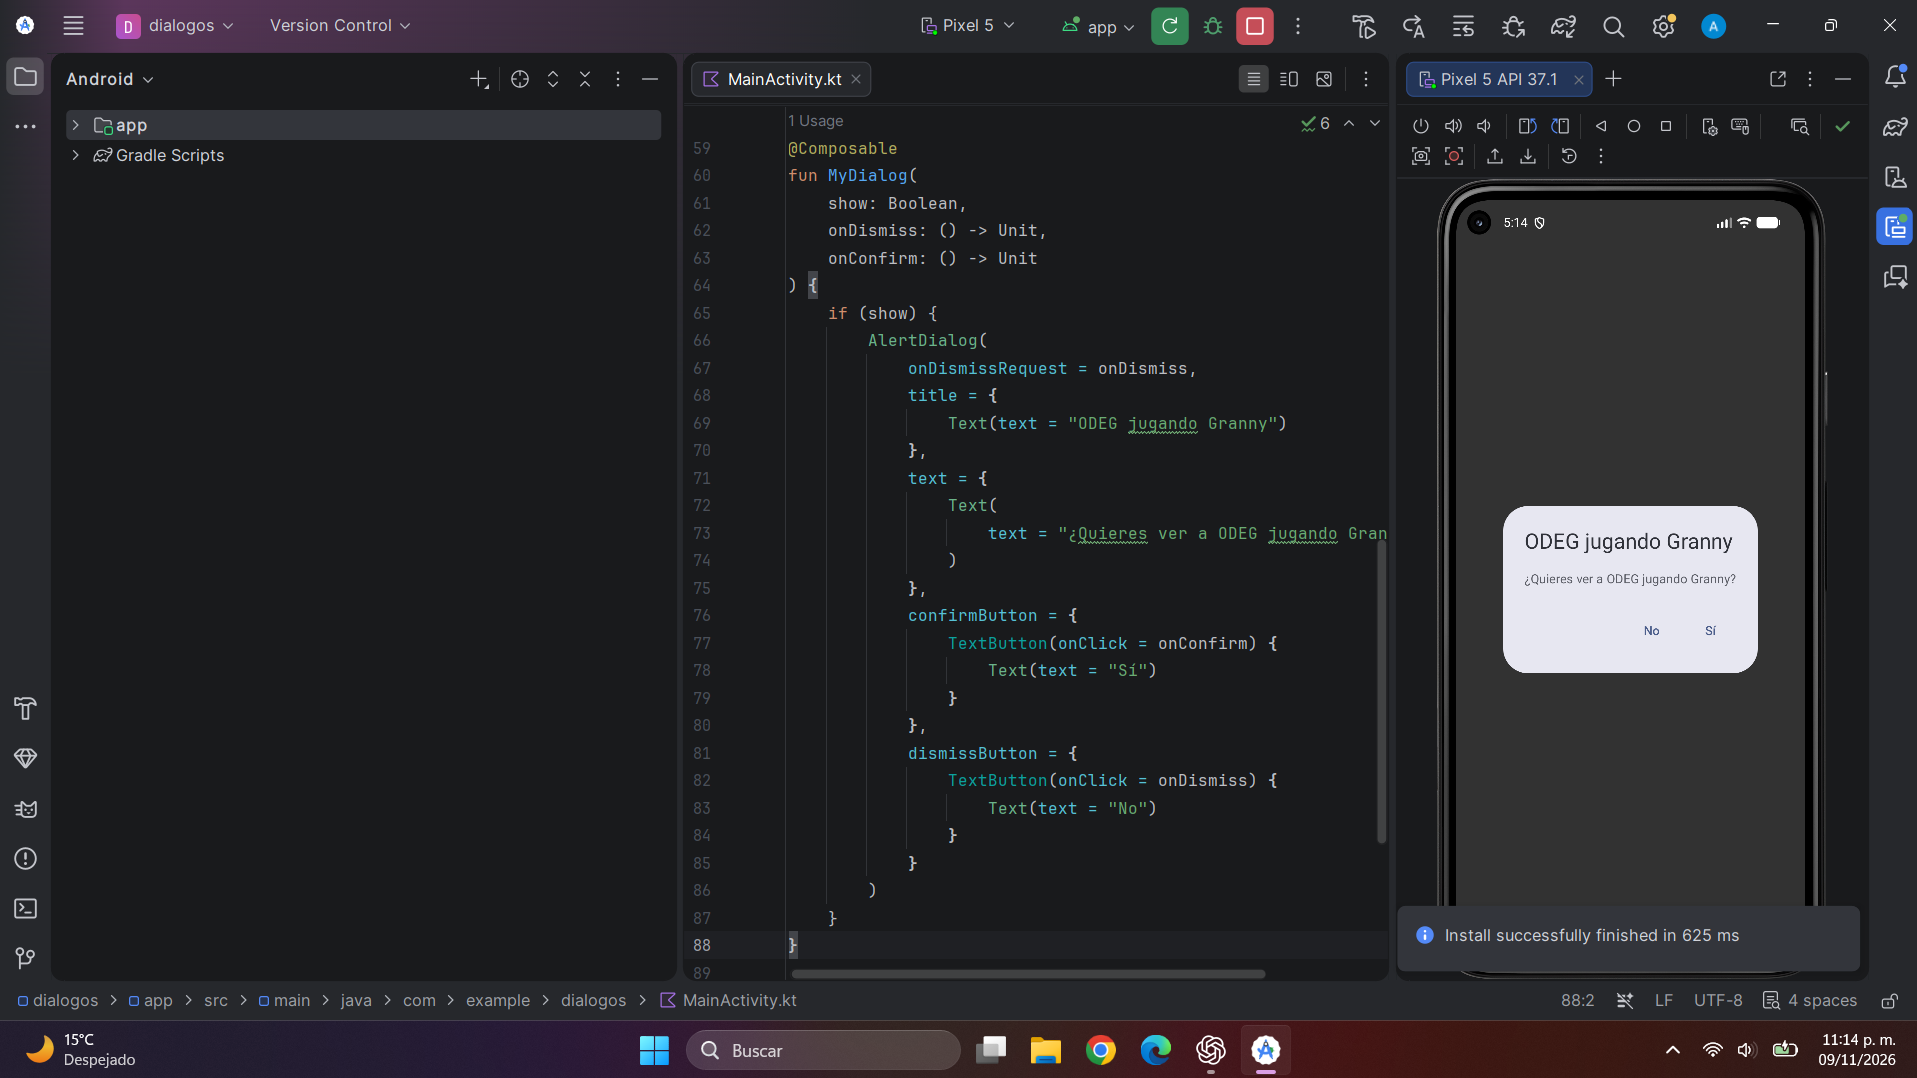
\includegraphics[width=\textwidth]{figura_10.png}
  \caption{Diálogo final}
\end{figure}

\section{Conclusiones}

El desarrollo de esta práctica permitió construir un diálogo de confirmación completo mediante Jetpack Compose y Material 3. Se comprobó que AlertDialog proporciona espacios definidos para el título, el mensaje y las acciones, facilitando la presentación de una decisión sin abandonar la pantalla principal.

Asimismo, remember y mutableStateOf permitieron controlar la visibilidad del componente. La pantalla conserva un valor booleano y lo modifica como respuesta a los eventos del usuario. Cuando el valor cambia, Compose actualiza la interfaz y muestra u oculta el cuadro según la condición declarada.

Finalmente, el uso de funciones para onDismiss y onConfirm permitió separar la presentación del diálogo de las acciones que modifican el estado. La ejecución en el emulador confirmó que el botón abre el cuadro, que No lo cierra y que Sí registra la confirmación antes de regresar a la pantalla inicial.

\section{Recomendaciones}

Se recomienda mantener el estado fuera del componente visual cuando la pantalla principal necesita controlar su comportamiento. Esta separación facilita reutilizar el diálogo con otros mensajes o acciones sin modificar su estructura interna.

También conviene conectar onDismissRequest aunque exista un botón de cancelación. De esta manera, el usuario puede cerrar el cuadro al tocar fuera de él o utilizar la acción Atrás, manteniendo un comportamiento esperado dentro de Android.

Por último, se recomienda compilar y ejecutar la aplicación después de cada cambio importante. Las pruebas en el emulador permiten comprobar la apertura, el cierre y la confirmación, mientras que Logcat ayuda a verificar acciones que no producen un cambio visual directo.

\clearpage
\section{Anexos}

\begingroup
\setlength{\parindent}{0pt}
\setlength{\parskip}{12pt}

\entradafrancesa{\textbf{Anexo A. Video tutorial consultado.} Programación by AristiDevs. (s. f.). \textit{Diálogos en Jetpack Compose} [Video]. YouTube. \url{https://www.youtube.com/watch?v=2rCyXaYkTp0&list=PL8ie04dqq7_ORKWIwiaSTcyBKtasZtNUD&index=8}}

\endgroup

\clearpage
\section{Referencias}

\begingroup
\setstretch{1.5}
\setlength{\parindent}{0pt}
\setlength{\parskip}{12pt}

\entradafrancesa{Android Developers. (2026a). \textit{Dialog}. Google. \url{https://developer.android.com/develop/ui/compose/components/dialog}}

\entradafrancesa{Android Developers. (2026b). \textit{Button}. Google. \url{https://developer.android.com/develop/ui/compose/components/button}}

\entradafrancesa{Android Developers. (2026c). \textit{State and Jetpack Compose}. Google. \url{https://developer.android.com/develop/ui/compose/state}}

\entradafrancesa{Android Developers. (2026d). \textit{Compose UI Architecture}. Google. \url{https://developer.android.com/develop/ui/compose/architecture}}

\endgroup

\end{document}
